

\documentclass{article}
\usepackage[utf8]{inputenc}
\usepackage{authblk}
\usepackage{setspace}
\usepackage{natbib}
\usepackage{hyperref}
%\usepackage{cite}
\usepackage[margin=1in]{geometry}
\usepackage{array}
\usepackage{graphicx}
\usepackage{caption}
\graphicspath{ {./figures/} }
\usepackage{subcaption}
\usepackage{gensymb}
\usepackage{amsmath}
\usepackage{lineno}
\usepackage{soul}
\usepackage{xcolor}
\sethlcolor{yellow}
\parindent=0pt
\linenumbers

%%%%%%%%%%%%%%%%%
\title{Does age matter in tree growth responses to longer growing season?} %emwJan2 -- you should start thinking of a title
\date{\today}
\author{Christophe Rouleau-Desrochers}

\begin{document}
%%%%%%%%%%%%%%%%%%%%%%%%%%%%%%

\maketitle

%<><><><><><><><><><><><><><><><><><><><><><><><><><><><><><><><><><><><><><><><>
% INTRODUCTION %
%<><><><><><><><><><><><><><><><><><><><><><><><><><><><><><><><><><><><><><><><>
\section*{Introduction}
% <><><><><><><><><><><><><><><><><><><><><><><><><><><><><><>
% SECTION 1.1. %
% <><><><><><><><><><><><><><><><><><><><><><><><><><><><><><>
\subsection*{Climate change impacts on tree phenology}
Research from the past decades has shown convincing evidence that human activity is increasingly affecting many worldwide environmental processes \citep{ceballos_biological_2017,intergovernmental_panel_on_climate_change_climate_2023,laurance_have_2007,parmesan_globally_2003}. 
This can be through land use change and loss, pollution, invasive species, resource overexploitation and climate change \citep{driscoll_biodiversity-crisis_2018,parmesan_poleward_1999,wu_key_2013}. Though some immediate actions can mitigate these impacts \citep[e.g.][]{campbell_producing_2014}, reversing 150 years of human-induced greenhouse gas emissions is harder. These emissions have affected Earth's climate and are projected to keep changing it for many centuries \citep{intergovernmental_panel_on_climate_change_climate_2023}. Yet, the extent of the consequences that a warming climate will have on biological processes is still debated \citep{huey_predicting_2012}, in part because it requires accurate predictions of current and future trends in some of the most reported and direct biological impacts of climate change, as I review below. And also because it requires understanding the complex additional effects of these impacts, which I propose to study for my thesis. \\

% <><><><><><><><><><><><><><><><><><><><><><><><><><><><><><>

% <><><><><><><><><><><><><><><><><><><><><><><><><><><><><><>
\textbf{Trends and drivers of spring and autumn phenological events} \\ 
The most frequently observed biological impact of climate change over the past decades is major changes in phenology---the timing of recurring life history events                                                                                                                                                                                                                                                                                                                                                                                                                                     \citep{parmesan_globally_2003,cleland_shifting_2007,lieth_phenology_1974,woolway_phenological_2021,menzel_european_2006}.  Shifts in spring and autumn phenology modify when the growing season starts and when it ends. These shifts in growing season length could have impacts on ecosystems and anticipating these consequences requires understanding how much, and why it has changed \citep{duputie_phenological_2015}. \\ 

\textit{Drivers of spring phenology:} Spring phenological events (e.g. budburst and leafout) have been advancing from 0.5 \citep{wolfe_climate_2005} to 4.2 days/decade \citep{chmielewski_response_2001,fu_recent_2014} and are mainly driven by temperature \citep{chuine_why_2010,cleland_shifting_2007,penuelas_responses_2001}, especially for trees. In the winter, when trees are still in dormancy, they accumulate cold temperatures (chilling) for which a certain amount is required to be ready to accumulate heat (forcing) \citep{vitasse_interaction_2014}. Then, in the spring, a certain amount of forcing triggers budburst \citep{fu_declining_2015}. Heat requirements are met sooner in warm springs, thus explaining the advancement of spring events and earlier onset of growing seasons over the last decades \citep{fu_declining_2015,fu_sensitivity_2013, laube_chilling_2014}. \\ 

\textit{Drivers of autumn phenology}: In contrast, autumn phenology (e.g. budset and leaf senescence) has delayed with climate change---though shifts in the autumn have been much smaller than those in the spring \citep{gallinat_autumn_2015,jeong_macroscale_2014}---and its drivers are also far less understood. Two realities could explain these differences: lesser attention is paid to autumn phenology \citep{piao_plant_2019} and the data is often noisier \citep{wu_canopy_2024}. However, some of these disparities are likely due to different factors driving autumn phenology, as these phenophases appear to be caused by shortening photoperiod and colder temperatures \citep{cooke_dynamic_2012,flynn_temperature_2018,korner_phenology_2010,delpierre_temperate_2016}. Given that low temperatures can accelerate senescence, warmer autumns may delay autumn phenophases, possibly by extending the activity of photosynthetic enzymes, which decreases the degradation rate of chlorophyll \citep{yan_divergent_2021}. Additionally, summer droughts could pause the activity schedule of trees and delay senescence to increase carbon assimilation \citep{dox_severe_2022}. Finally, there could be other factors affecting senescence delays that we do not consider here, such an antagonistic effect of warming and atmospheric brightening \citep{sanchezlorenzo_reassessment_2015,wu_atmospheric_2021}. \\

% <><><><><><><><><><><><><><><><><><><><><><><><><><><><><><>
\textbf{How shifts in spring and autumn phenology will affect trees and forests are not clear} \\ 
Shifts in spring and autumn phenology in trees support a long-lasting and intuitive assumption that earlier spring and delayed autumn events extend seasons and thus increase growth \citep{keenan_net_2014, stridbeck_partly_2022}. However, research from recent years has cast doubt on this hypothesis \citep{dow_warm_2022,green_limits_2022,silvestro_longer_2023}. For instance, \cite{dow_warm_2022} showed that despite an earlier growth onset, longer seasons did not increase the growth rate nor overall annual increment in trees. This could substantially affect forest carbon-cycle model projections on and thus feedbacks to future climate \citep{richardson_climate_2013,swidrak_comparing_2013}. These projections are likely to be furtherly altered by the different effects that an earlier start and a later end of season have on trees, some of which I propose to study in this thesis (Figure \ref{fig:effects}). \\

% --- --- --- --- --- --- --- --- --- --- --- --- --- --- --- ---
% Effect figure %
% --- --- --- --- --- --- --- --- --- --- --- --- --- --- --- ---
\begin{figure}[h!]
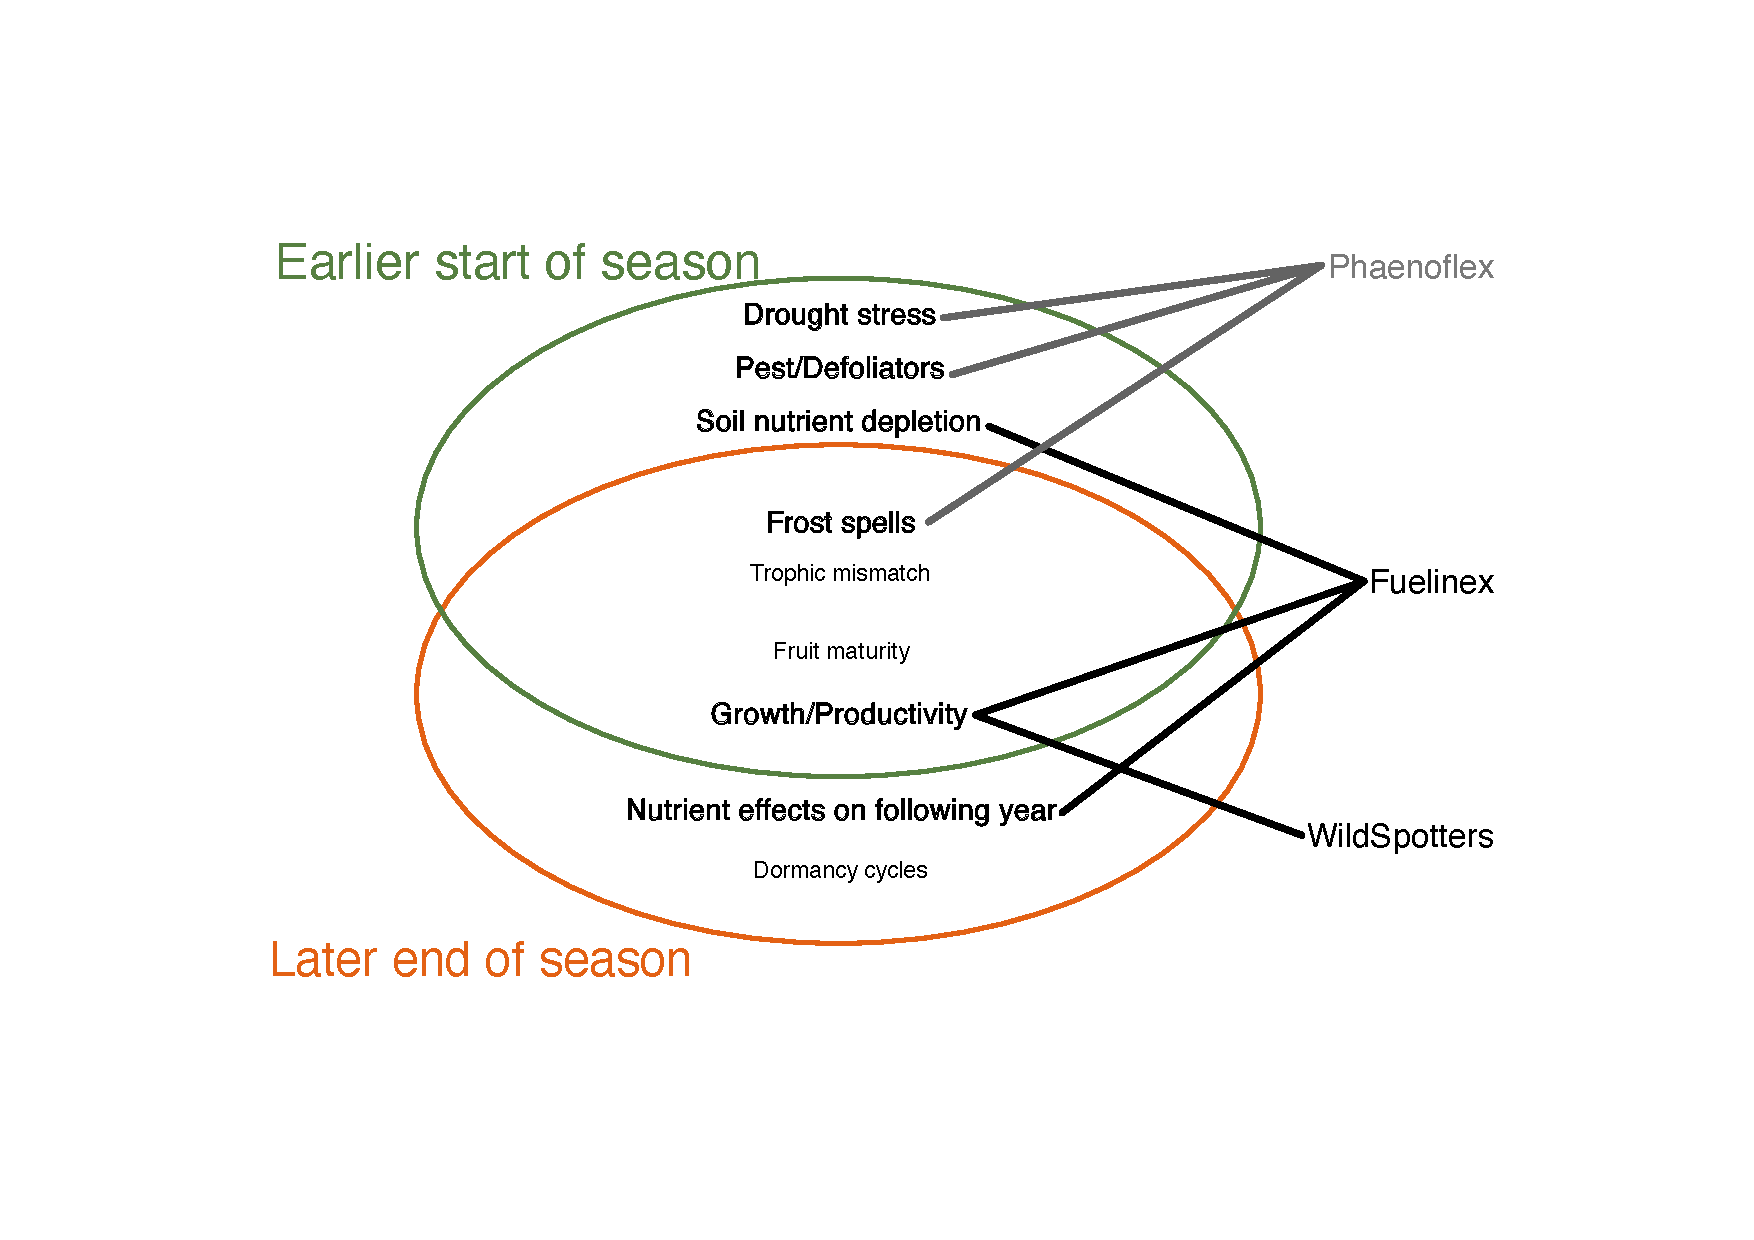
\includegraphics[width=0.5\textwidth]{studiedEffectsGSL.pdf}
\caption{The effects that an earlier start and later end of season can have on trees. Solid lines connect effects studied over the course of this thesis. Phaenoflex (in grey) and its dashed lines represent other effects I investigated in a related experimental project that is not part of this thesis, but one I collaborated on in 2023 and 2024. }
\label{fig:effects}
\end{figure}

Understanding these findings requires answering why trees do not grow more despite longer growing seasons. While carbon allocation to above-ground biomass is one of the largest carbon sinks, how this carbon is allocated into wood is poorly understood. Indeed, the assumption of a linear relationship between wood growth and carbon assimilation is not well supported mechanistically and represents an important limitation of vegetation models \citep{cabon_cross-biome_2022}. Net primary production represents the difference between photosynthesis and plant respiration, but this commonly used metric omits the representation of growth processes. This is perhaps because of a long-lasting paradigm of source-limited photosynthesis \citep{friend_need_2019,parent_modelling_2010}. Whether a tree's growth is source (photosynthetic activity determines sink activity) or sink (growth, respiration, and other metabolic processes determine the carbon source) controlled depends upon a closely coordinated sequence of dynamic responses and is still an active research question. However, \cite{gessler_beyond_2024} recently suggested that neither source nor sink control systematically dominates. This complex dynamic enforces the importance of understanding the temperature sensitivity relationship between growth activity and photosynthesis. Growing evidence suggests that cambial activity may be more sensitive than photosynthesis to a range of environmental conditions, such as water and nutrient availability, and temperature \citep{cabon_cross-biome_2022,cabon_water_2020,muller_water_2011,peters_turgor_2021}. Thus, this demonstrates that carbon projection models that solely rely on vegetation alone may mislead carbon sequestration dynamics of our forests. \\

Spring and fall phenological events are shifting with debatable consequences on tree growth. The sensitivity of cambial activity to water, temperature and nutrients has the potential to have far-reaching consequences given the hard-to-predict nature of future climate change, where any of these variables could vary from low to high amplitude \citep{almagro_longterm_2025,cabon_cross-biome_2022}. This expected asymmetry of future environmental changes makes understanding the internal physiological constraints (via genetic and developmental control), and external limits (via extreme temperatures or moisture deficit) to growth critical, which I aim to investigate with experiments and observations. 

% <><><><><><><><><><><><><><><><><><><><><><><><><><><><><><>
% SECTION 1.2 %
% <><><><><><><><><><><><><><><><><><><><><><><><><><><><><><>
\subsection*{Experiments and observations to anticipate the future of growth and season length relationship} 
\textbf{Past phenological trends can help (or not) predict future phenological changes} \\ 
We cannot directly use observed phenological trends in the last decades to extrapolate future phenological changes because: (1) the mechanisms guiding them are not clear, and (2) phenological responses of trees to warming are very likely to be non-linear \citep{ettinger_winter_2020,fu_sensitivity_2013}. Indeed, accurate predictions require an in-depth mechanistic understanding of phenophases and their sensitivities to environmental drivers, especially to temperature and photoperiod \citep{fu_sensitivity_2013}. Therefore, the very foundation of the assumption that longer seasons increase growth may shift with future climate change. The well-observed advance in spring phenology may decelerate, and delayed fall phenology may shift towards earlier leaf senescence (through summer drought-induced growth cessation). \\

\textbf{Growth drivers differences across species need to be considered} \\ 
Recent work emphasizing the need to understand the drivers regulating growth across biomes highlights strong species-level variation that may be critical to accurate projections. Phenology varies greatly across species \cite[e.g., closely related species tend to budburst at similar times under similar conditions][]{wolkovich_progress_2014}, but so does the relationship between growth and season length, which may explain the wide variation of this relationship within communities \citep{buckley_functional_2012}. This points out another weakness of current carbon sequestration models that pool species together, likely missing important nuances in the growth responses plausibly explained by species differences. Excluding species differences in models may mislead future carbon dynamic models \citep{green_limits_2022,cabon_cross-biome_2022,wolkovich_why_2025}. We propose to adress this issue by using experiments and ground-based observations to better understand the responses of different species to warming. While both of these strategies have downsides, they are likely to leverage valuable insights which are necessary to improve carbon sequestration projections \citep{wolkovich_why_2025}. \\

\textit{Experiments:} First, experiments are extremely useful in teasing apart co-occurring realities in natural environments. For example, warm springs and severe droughts later in the summer often happen together within a single year, making it difficult to tease these effects apart from observational data. Manipulative experiments, in contrast, have the capacity to separate the relative effect of each phenomenon \citep{morin_changes_2010,primack_observations_2015}, but also have major limitations, especially when working on trees. Logistical constraints of working with adult trees mean that experiments are most often performed on juvenile trees. While saplings are critical for their role in forest regeneration projections, their responses often do not directly translate to mature trees, which hold the overwhelming carbon biomass proportion of forests \citep{augspurger_differences_2003,silvestro_longer_2023,vitasse_ontogenic_2013}. However, even if young trees are often more plastic than adult forms, their responses can still provide valuable insights into differences across species and populations \citep{wolkovich_why_2025}. \\

\textit{Ground-based observations:} 
Second, leaf phenology can provide valuable and accessible insights into the growth temporality of trees that are not suitable for experimental trials. Collecting cambial phenology data, which is a direct measure of wood growth, is time-consuming and expensive. In contrast, leaf phenology through ground-based observations are low-cost methods that provide direct evidence of changing phenophases \citep{piao_plant_2019}. Cambial and leaf phenology are often closely synchronized \citep{stridbeck_partly_2022}; therefore, the more accessible leaf phenology data can act as a reliable proxy for the onset and end of tree growth. In other words, knowing when leaves elongate and colour can guide as to when trees start and stop growing, which is a fundamental metric to determine the growing season length. Additionally, unlike other methods, ground observations have the advantage of providing accurate measurements of phenological events for specific sites and species. Recently, the widespread use of smartphones has considerably simplified the phenological monitoring by citizen scientists \citep{dickinson_current_2012,hufkens_monitoring_2019,piao_plant_2019}. While there are drawbacks to observations by citizen science programs (e.g. non-standard protocols, highly uneven spatiotemporal distribution of these observations), they have the potential to vastly increase the range of studied species and areas \citep{chandler_contribution_2017,feldman_how_2018}. \\
 
\textbf{Goals of my thesis}  \\ 
I aim to understand how different tree species, at different lifespan stages, vary in their growth responses to different season lengths. To achieve this, I worked across different methods (Figure \ref{fig:chaptersDesign}). First, I deployed a large-scale experiment, named Fuelinex, during which I artificially controlled the growing season length for seven species of tree saplings (2-3 years old). During this experiment, I also tested nutrient effects later in the season. Second, I leveraged observational data from older trees across two projects. One of them, which I named Wildchrokie, leverages vegetative phenology data from a common garden project of four species of juvenile trees (5-8 years old). With the other observational project, named coringTreespotters, I used phenology data collected by citizen scientists on eleven species of fully mature trees ($>$30 years old). With these projects, I hope to explain the growth patterns of trees, but it requires defining growth and the growing season.

% <><><><><><><><><><><><><><><><><><><><><><><><><><><><><><>
% SECTION 1.3. %
% <><><><><><><><><><><><><><><><><><><><><><><><><><><><><><>
\subsection*{Complexity of measuring growth and defining growing season length} 

\textbf{What is a growing season?} \\
The definition of the growing season itself is not well-defined, and studies use an array of definitions. Recently, \cite{korner_four_2023} proposed four definitions addressing this issue: (1) true growing season, based on measurable growth; (2) phenological season, based on visible phenological markers; (3) the productive season, based on primary production and (4) meteorological season, based on environmental conditions.

Here, I will focus on how the phenological season (2), incorporating the (4) meteorological season, affects the true growing season (1) as our data cannot address the productive season (3). I will use the phenological season (2) to infer a "window of opportunity", to calculate growing degree days (GDD)---a measure of heat accumulation---using meteorological conditions. \\

\textbf{What is growth?} \\ 
Wood formation (xylogenesis) consists of allocating carbon for long-term storage in woody plants. Xylogenesis starts with cambial activation and cell production, which produces xylem and phloem cells
\citep{etzold_number_2022,silvestro_roots_2025}. The rate and duration of these phases lead to irreversible radial growth increments usually represented through tree rings \citep{plomion_wood_2001,rathgeber_biological_2016}. \\

Foresters have measured tree diameter and height for decades, but these measurements may not be suitable for determining relationships between growth and environmental conditions. 
The widely used method in forestry is to measure diameter at breast height at punctual time intervals. Combined with height, these data help develop allometries foresters can use to estimate how much wood they can harvest in a forest \citep[e.g.,][]{meyer_mathematical_1940,saunders_height-diameter_2008}. These metrics work to determine wood in forests, but their coarse temporal scale---measuring every 5 or more years--- is likely to miss extreme events affecting growth. \\

Alongside the diameter-height allometric relationship, dendroecology---applications of dendrochronological techniques to problems in ecology \citep{fritts_dendroecology_1989}---emerged to answer ecological problems as well as to hindcast \citep[e.g.,][]{bergeron_fire_2004}) and forecast ecological processes both at the regional \citep{gazol_forest_2018} and global scale \citep{manzanedo_towards_2019, buntgen_tree_2018}. Now, these methods can unveil more precise growth patterns and their relationship with different environmental factors. This is why I will use tree rings as a proxy for how much trees grew in any given year.\\

% <><><><><><><><><><><><><><><><><><><><><><><><><><><><><><>
% SECTION 1.4. %
% <><><><><><><><><><><><><><><><><><><><><><><><><><><><><><>
\subsection*{Objectives}  
The objectives for my experiment (Fuelinex) are to assess tree species’ potential to prolong or stretch their activity schedule by artificially manipulating growing season length and analyze how this translates (or not) into growth, during the current year (2024) and in the following year (2025). I will also conduct a secondary experiment to examine whether trees can absorb nutrients late in the season and if that translates into growth during the following season. For the observational data projects (Wildchrokie and coringTreespotters), I will investigate how the timing of phenological events affects growth across years for juvenile and mature trees, using observational phenology data and tree rings. The duration and type of study, the age classes and species used in each project are presented in Figure \ref{fig:chaptersDesign}). Together, my two chapters will allow me to investigate the decoupling between growth increment in response to longer growing seasons. 
 
% --- --- --- --- --- --- --- --- --- --- --- --- --- --- --- ---
% Thesis overview figure %
% --- --- --- --- --- --- --- --- --- --- --- --- --- --- --- ---
\begin{figure}[h!]
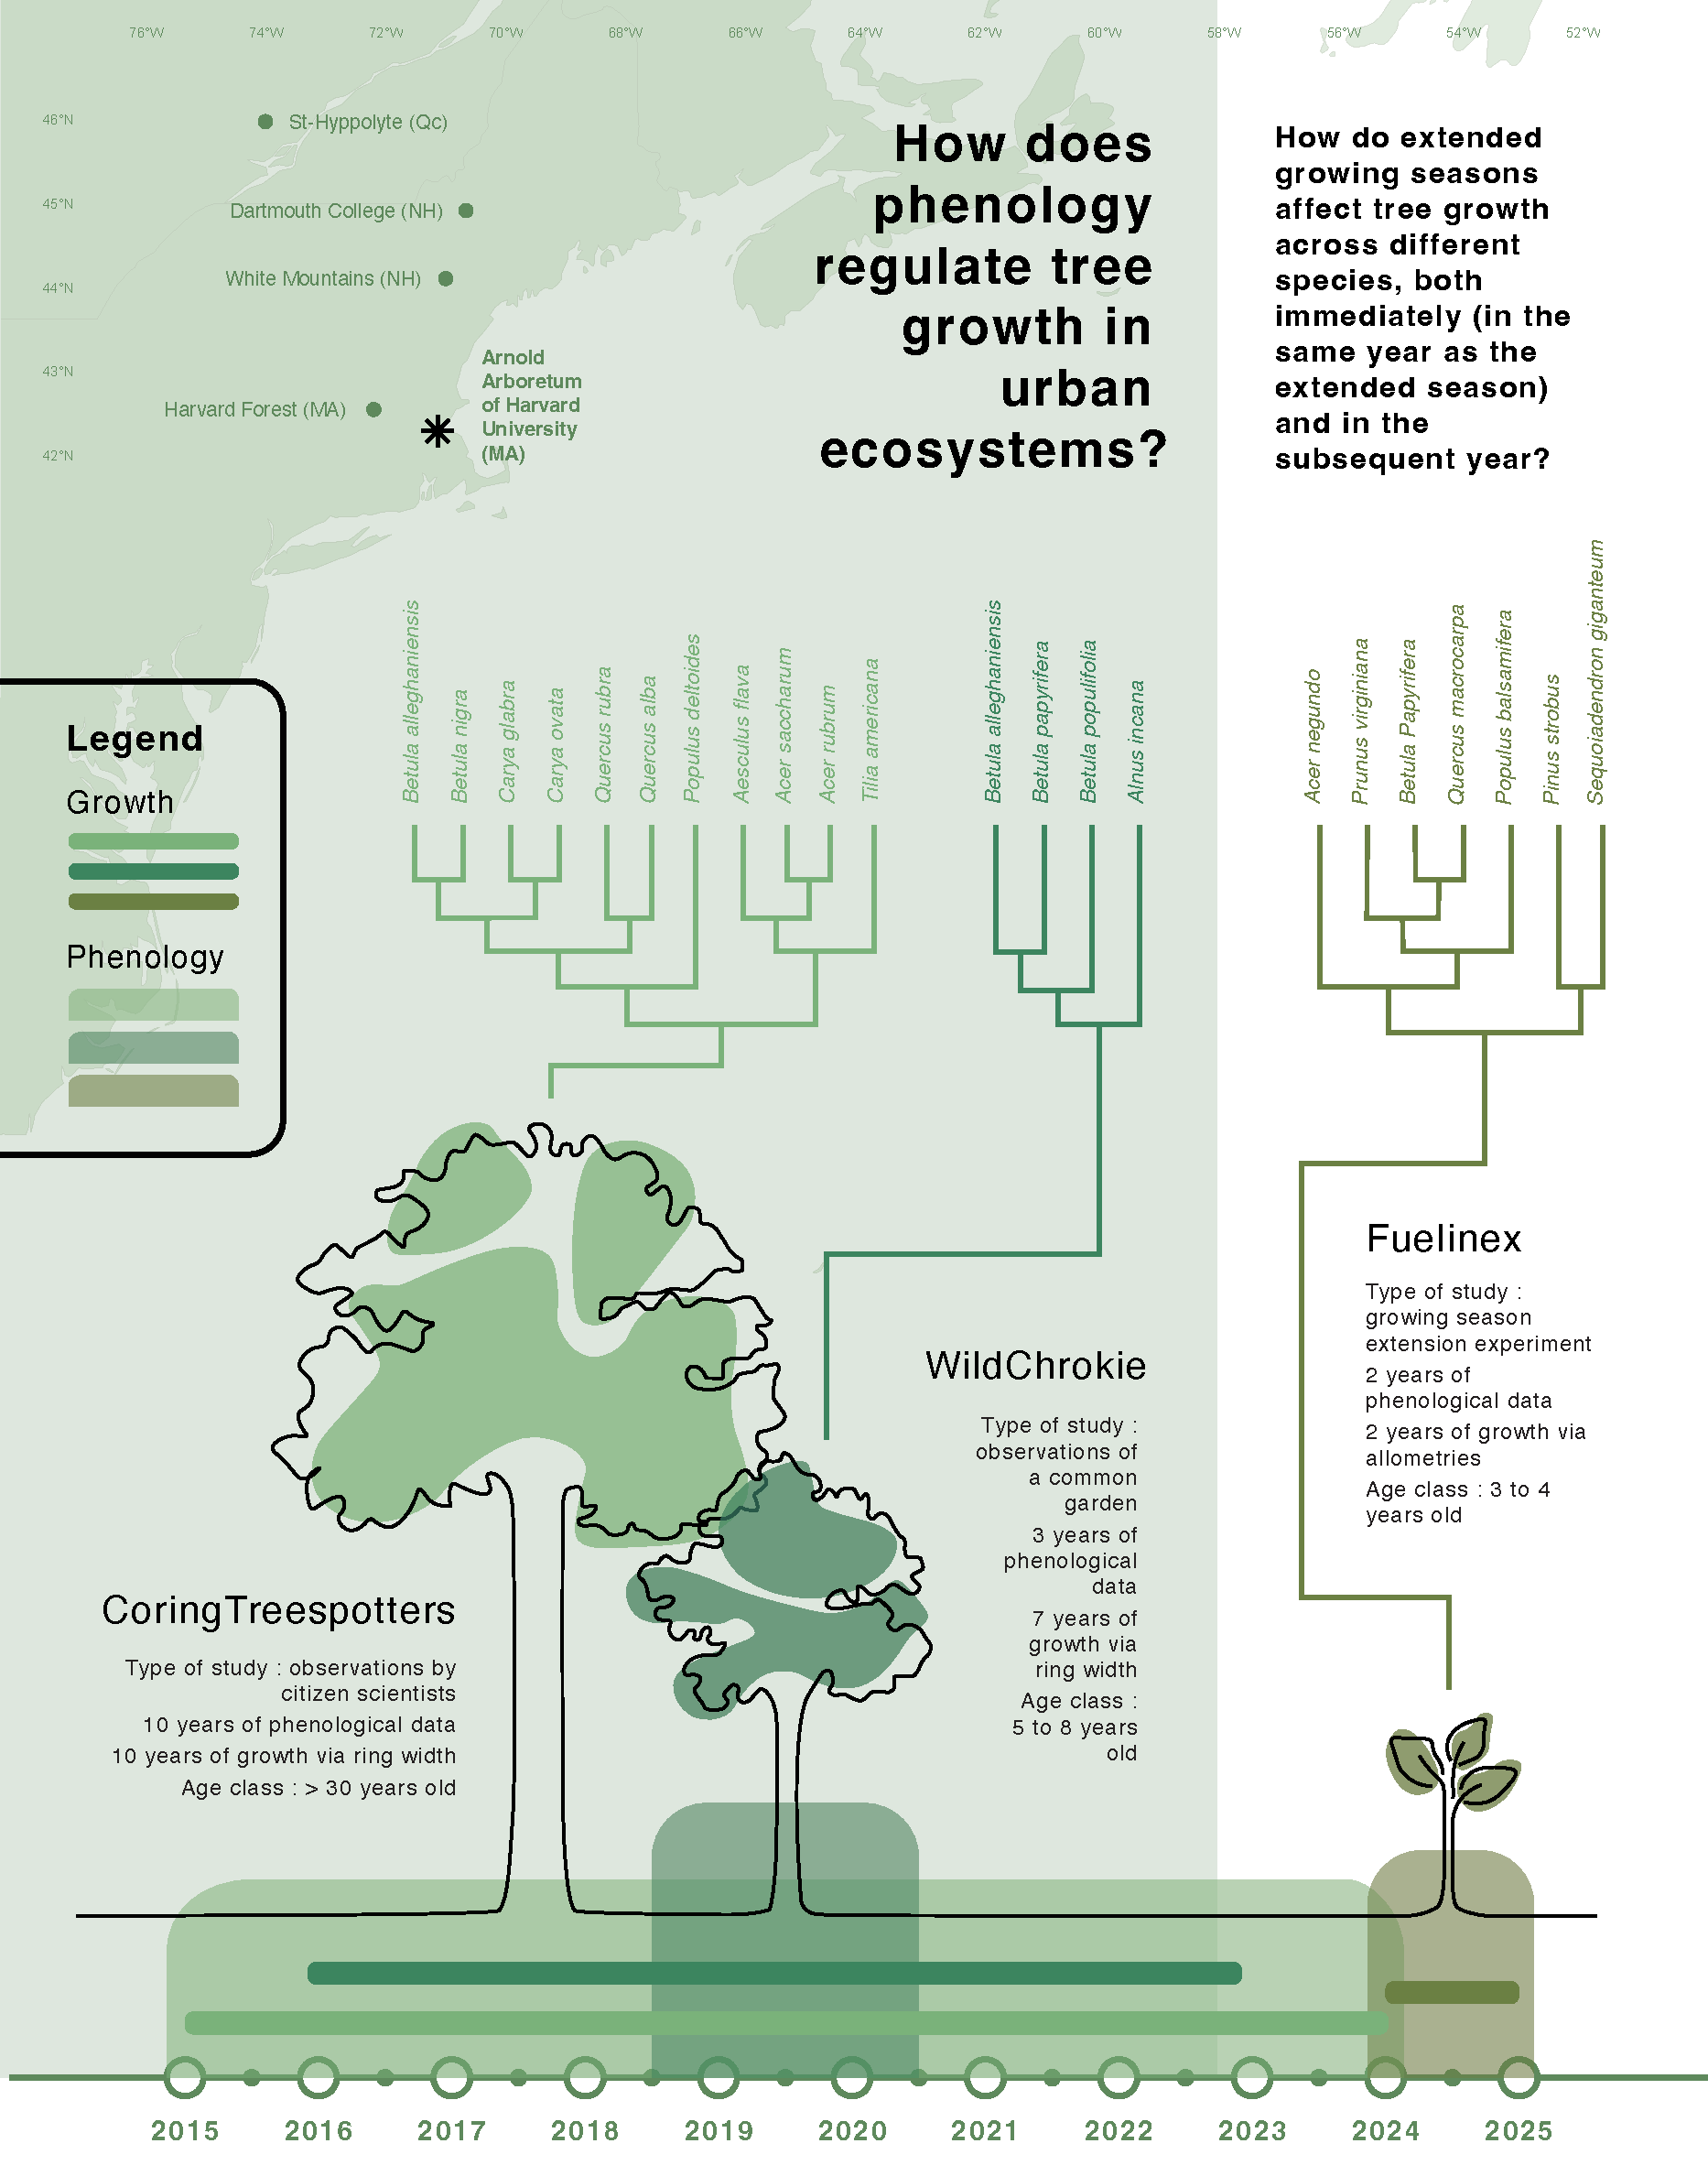
\includegraphics[width=0.7\textwidth]{chaptersDesign.pdf}
\caption{Overview of the age class, species, provenance of the trees used in each study along with the type of study each project consist of. The colored lines represent the period of the growth data and the shaded ared, the phenological data. Each phylograms illustrate the species used in each project. The map illustrate the four different provenances used in Wildchrokie and the start represents the location of Wildchrokie and coringTreespotters.}
\label{fig:chaptersDesign}
\end{figure}

% <><><><><><><><><><><><><><><><><><><><><><><><><><><><><><>
% SECTION 1.5. %
% <><><><><><><><><><><><><><><><><><><><><><><><><><><><><><>
\subsection* {Research questions} 
{Fuelinex}: How do extended growing seasons affect tree growth across different species, both immediately (in the same year as the extended season) and in the subsequent year?
{Wildchrokie and coringTreespotters}: How does phenology regulate tree growth in urban ecosystems? \\

%<><><><><><><><><><><><><><><><><><><><><><><><><><><><><><><><><><><><><><><><>
% METHODOLOGY %
%<><><><><><><><><><><><><><><><><><><><><><><><><><><><><><><><><><><><><><><><>
\section*{Methodology} 

% <><><><><><><><><><><><><><><><><><><><><><><><><><><><><><>
% FUELINEX %
% <><><><><><><><><><><><><><><><><><><><><><><><><><><><><><>
\subsection* {Chapter 1: Fuelinex}

\textbf{Species selection and growing conditions}
We used seven species of tree saplings for our experiment (Fuelinex). We purchased Paper birch (\textit{Betula papyfera}), Choke Cherry (\textit{Prunus virgiana}), Bur oak (\textit{Quercus macrocarpa}) from Peel's nursery in November 2023 and the trees arrived at Totem Field studios (49.26 \degree N, -123.25 \degree W), where the other four species were stored until the spring of 2023. Manitoba maple (\textit{Acer negundo}), Eastern white pine (\textit{Pinus strobus}), Balsam poplar (\textit{Populus balsamifera}) and Giant sequoia (\textit{Sequoiadendron giganteum}) were leftover trees that we purchased in 2022 for 2023 for a previous experiment. We watered them weekly, and they remained at ambient conditions for the 2023 growing season. We randomly selected 90 individuals of each species among them. We propagated \textit{P. balsamifera} from 30 cm whips while the trees were still dormant \citep{mc_carthy_early_2018}. In May 2024, we repotted all the trees in 2-gallon plastic pots with a medium for perennials consisting of 50 \% peat, 25\% crushed pumice and 25\% crushed bark (purchased from www.westcreekfarm.com). In February 2025, we repotted the trees with the same medium in 3-gallon pots. We arranged the trees in three blocks, each containing all 6 treatments and 7 species, with two of these blocks placed under an open-walled and well-ventilated polytunnel greenhouse. All saplings were connected to a drip irrigation system (40 PVC frame from Netafilm 54 with a Toro controller) to maintain constant irrigation across the season. Using fertilizer premix, we fertilized the trees twice during the growing season of 2024 (except for the nutrient-boosted trees) and three times during 2025, just enough to keep the trees alive (Table \ref{tab:nutrient}). \\

\textbf{Tree measurements and biomass}: \\
Using red paint, we marked the trees on their trunk at ~3 cm from the soil in February 2024. Then we measured the diameter at the top of that mark using a digital calliper (accuracy $\pm$ 0.01cm). From that mark to the bottom of the highest apical bud, for angiosperms, and the top of the apical meristem for gymnosperms, we measured height with a metal ruler (accuracy $\pm$ 0.1cm). We measured those two same points in the winter (2024 growing season) and in the fall (2025 growing season) of 2025. For those two subsequent measurements, if the measured shoot died (because of insects, accidentally snapped off, etc.), we noted the previous measurement as invalid and measured the highest lateral shoot. In the fall of 2025, when all the individuals from a species had lost all their leaves, we removed the trees from their pots and gently washed the soil off the roots with a water hose. We dried the trees by placing them in drying ovens at 70\degree C for 72 hours and weighed the roots and stem separately (accuracy $\pm$ 0.01 gram). \\

\textbf{Phenology and shoot elongation monitoring}: \\
\textit{Leaf phenology}: We started monitoring phenology of all the trees on 11 April 2024, missing the initial leaf phenology for most individuals, but we monitored subsequent phenophases twice a week until the leaves had fully elongated. In the late summer and fall, we monitored budset every week until full bud dormancy. Phenophases are described in Table \ref{tab:phenostages}. Phenophases of \textit{S. giganteum} were not recorded. \\

\textit{Shoot elongation}: Before shoot elongation onset, we marked a reference point with red paint at the base of either the new-year apical or the highest lateral shoot. To facilitate and improve the quality of the shoot elongation measurements, we attached paper rulers (accuracy $\pm$ 0.1cm) on \text{A. negundo, B. papyfera, P. balsamifera} and \textit{Q. macrocarpa}. For species not suitable for those paper rulers, we took those same measurements, but with a metal ruler (accuracy $\pm$ 0.1cm). We measured shoot elongation weekly from the red mark to the base of the bud for angiosperms, and at the top of the apical meristem for gymnosperms. For determinate growth species ( \textit{A. negundo, P. virgiana} and \textit{Q. macrocarpa}), when the trees did not elongate for two weeks, we started monitoring them every other week until September 1st for both growing seasons. \\

\textit{Senescence}: Every week, starting on 4 September 2024, we monitored senescence by a visual assessment of the remaining green leaf cover in percentage and by measuring the chlorophyll content meter with a SPAD-502 chlorophyll meter (Minolta Camera Co. Japan). We also recorded the date of loss of green leaf cover and leaf drop. \\

% --- --- --- --- --- --- --- --- --- --- --- --- --- --- --- ---
% PHENOSTAGE TABLE
% --- --- --- --- --- --- --- --- --- --- --- --- --- --- --- --- 
\begin{table}[h!]
\centering
\caption{Phenological stages and their descriptions for deciduous species and pine (From Baumgarten, unpublished) and \citep{vitasse_ontogenic_2013}}
\renewcommand{\arraystretch}{1.2}
\begin{tabular}{cllp{8cm}}
\hline
\textbf{Group} & \textbf{Scale} & \textbf{Phenostage} & \textbf{Description} \\
\hline

\multicolumn{4}{l}{\textit{Deciduous species}} \\
0 &  & dormant & no bud development visible \\
1 &  & bud swelling & swollen and/or elongating buds \\
2 &  & budburst & bud scales open and leaves partially visible \\
3 &  & leaf-out & leaves fully emerged from bud but still folded, crinkled or pendant \\
4 &  & leaf unfolding & leaves fully unfolded \\

\hline
\multicolumn{4}{l}{\textit{Pine}} \\
0 &  & dormant & no signs of activity \\
1 &  & swelling & swelling or elongation of shoot visible \\
2 &  & budburst & green needle tips along the shoot visible \\
3 &  & leaf-out & scales open along the shoot and first needles become visible \\
4 &  & leaf-unfolding & green needles emerging away from the shoot \\

\hline
\end{tabular}
\label{tab:phenostages}
\end{table}


\textbf{Experimental design}
Individuals from each species were randomly selected for a full factorial design of Warm/Cool, Spring/Fall treatments (Figure \ref{fig:fuelinexFactorial}) with two additional treatments to test nutrient effects in the fall (Figure \ref{fig:fuelinexDesign}), for a total of 15 replicates/treatment/species. On 6 March 2024, we placed the Cool Spring individuals in climate chambers to delay the start of their growing season, while the Warm Spring replicates remained at ambient conditions. Once all Warm Spring individuals had fully leafed out, we removed the Cool Spring replicates from the chambers and placed them back at ambient conditions for the whole summer. On 4 September 2024, we placed the trees for the Warm Fall treatments in the climate chambers. The temperature was set to fit the mean 30-year weekly maximum temperature of the previous month (e.g. 1st week of September set to the average of the 1st week of August). The Cool Fall treatment trees remained at ambient conditions. For both climate chamber treatments, we rotated and watered the trees weekly to minimize the climate chamber's effect. We also set the photoperiod regime to the corresponding sunrise and sunset of the ongoing week and ramped it until it reached full light. To test for nutrient limitation at the end of the season, we added a supplemental dose of nutrients (Table \ref{tab:nutrient}) to two treatments (Figure \ref{fig:fuelinexDesign}). In 2025, all the trees were kept at ambient conditions together at Totem field during which we recorded the same phenophases.\\

\textbf{Leaf count}
To determine if nutrient addition treatments in the fall affected leaf primordia formation, we counted the apical meristem leaves on 27 May 2025 for the determinate growth species only (\textit{A. negundo, P. virgiana} and \textit{Q. macrocarpa}). 

\clearpage
% --- --- --- --- --- --- --- --- --- --- --- --- --- --- --- ---
% 2024 Experimental design %
% --- --- --- --- --- --- --- --- --- --- --- --- --- --- --- ---
\begin{figure}[h!]
\includegraphics[width=0.9\textwidth]{Fuelinex_Design2024.pdf}
\caption{Experimental design during the 2024 growing season. Cooling treatments are represented in blue, and warming treatments are in orange. The grey zone in the middle represents an approximate period during the growing season where all treatments were together at ambient conditions. The colored arrows represent the approximated periods during which we recorded the phenostages.}
\label{fig:fuelinexDesign}
\end{figure}


% <><><><><><><><><><><><><><><><><><><><><><><><><><><><><><>
% WILDCHROKIE %
% <><><><><><><><><><><><><><><><><><><><><><><><><><><><><><>
\subsection*{Chapter 2: Wildchrokie and coringTreespotters} 
\textbf{Wildchrokie} \\
\textit{Common garden setup (direct quote from Buonaiuto, in review)} \\
"In 2014-2015, we collected seeds from four field sites in northeastern North America spanning approximately a 3.5◦ latitudinal gradient. The four field sites included Harvard Forest (42.55 \degree N, 72.20\degree W), the White Mountains (44.11 \degree N, 71.40 \degree W), Second College Grant, (44.79 \degree N, 71.15 \degree W), and St. Hippolyte, QC, CAN (45.98 \degree N, 74.01 \degree W) (Figure \ref{fig:wildSpottersMap}). We transported all seeds back to the Weld Hill Research Building at the Arnold Arboretum in Boston Massachusetts (42.30 \degree N, 71.13 \degree W) where we germinated seeds following standard germination protocols, and grew them to seedling stages in the research greenhouse. In the spring of 2017, we out-planted seedlings to establish the garden. Plots were regularly weeded and watered throughout the duration of the study and were pruned in the fall of 2020." \\

% --- --- --- --- --- --- --- --- --- --- --- --- --- --- --- ---
% Map %
% --- --- --- --- --- --- --- --- --- --- --- --- --- --- --- ---
\begin{figure}[h!]
\includegraphics[width=0.9\textwidth]{mapSourcePop.jpeg}
\caption{Locations of the provenance study for the common garden study (Wildchrokie). The common garden and the citizen science project (coringTreespotters) took place at the Arnold Arboretum of Harvard University, represented by the orange star.}
\label{fig:wildSpottersMap}
\end{figure}

\textit{Phenological monitoring and sample collection (direct quote from Buonaiuto, in review)} \\
"For the years 2018-2019, we made phenological observations of all individuals in the common garden twice per week from February to December. In 2020 due to the COVID 19 pandemic, we monitored them once per week from March to November. We describe phenological stages using a modified BBCH scale, a common metric for quantifying woody plant phenological progression \citep{finn_general_2007}. We observed all major vegetative stages (budburst BBCH 07, leafout BBCH 15, end of leaf expansion BBCH 19, leaf coloration/drop BBCH 97, reproductive phases flowering BBCH 60-65, fruiting BBCH 72-79 and fruit/cones fully ripe BBCH 89). We added additional phases for budset and labelled the full budset as BBCH 102." In the spring of 2023, we collected cross-sections for most trees and 1 tree core on a few individuals. Both the cores and cross-sections were left to dry at ambient temperature for three months. \\

% <><><><><><><><><><><><><><><><><><><><><><><><><><><><><><>
% CORINGTREESPOTTERS %
% <><><><><><><><><><><><><><><><><><><><><><><><><><><><><><>
\textbf{Coringtreespotters} \\
\textit{Citizen science program} \\
The Treespotters was a citizen science program that started in 2015 and aimed to train citizen scientists for accurate and rigorous phenological monitoring at the Arnold Arboretum of Harvard University (42.30 \degree N, -71.12 \degree W) (Figure \ref{fig:wildSpottersMap}). From 2015 to 2024, hundreds of citizen scientists monitored 50 trees of 11 species. They regularly followed those individuals from budburst in the spring to leaf colouring in the fall using the National Phenology Netword (NPN) phenophases \citep{denny_standardized_2014}: Leaves (483), Colored leaves (498), Fruits (516), Ripe Fruits (390), Falling leaves(471), Recent fruit or seed drop (504), Increasing leaf size (467), Breaking leaf buds (371), Flowers or flower buds (500), Open flowers (501), Pollen release (502). Not all phenophases were recorded for every tree, for every year, and some trees miss several years of data. \\

\textit{Phenological monitoring and sample collection} \\
From 20 to 22 April 2025, we collected two 5-mm diameter cores, 15-cm length at 1.3 meters above ground from 50 trees of the 11 species (Table \ref{tab:coringTreespottersSpecies}) that were previously monitored for phenology, using an increment borer (Mora Borer, Haglöfs Sweden, Bromma, Stockholm, Sweden). We collected the cores perpendicular to the slope and at 180 degrees from each other, cleaning the increment borer with alcohol (70\% ethanol) and the inside with a brush before collecting each core. We stored the cores at ambient temperature for three months in paper straws that were previously labelled and punched to help with drying. \\

\textbf{Sample processing, imaging and measuring} \\
We mounted the cores on wooden mounts, and sanded the cores and cross-sections using progressively finer sandpaper (grits 150, 300, 400, 600, 800, 1000). We scanned the cores and cross-sections at a resolution of 6250 dpi, with a high resolution treering scanner (Fong, unpublished). We used the digitized images to measure the tree ring widths with ImageJ \citep{schneider_nih_2012}. Then, we performed visual crossdating using Dplr \citep{bunn_statistical_2010}, we did not perform statistical crossdating because of the short chronologies that limit the capacity of these analyses \citep{raden_potential_2020}. \\

\textbf{Statistical analyses} \\
For both projects, we used Bayesian hierarchical models coded in Stan with the rstan package version 2.32.7 \citep{carpenter_stan_2017} to run the Stan code in R. With these models, we estimated ringwidth as a function of growing degree days, accumulated from the leafout date to the budset date. We had three grouping factors for Wildchrokie (species, site and treeid) and two for coringTreespotters (species and treeid). We ran four chains with each 2000 warmup, which we discarded, and 2000 sampling iterations, which we kept for posterior distribution estimates. The models did not have any divergent transitions and $\hat{R}$ was below 1.01. \\

\textit{Wildchrokie model structure}
\[
\begin{aligned}
ringwidth_i &\sim \text{Normal}(\mu, \sigma_y) \\
\mu &= \alpha + \alpha_{\text{species}} + \alpha_{\text{site}} + \alpha_{\text{treeid}} + \beta_{species}* gdd \\
\alpha_{\text{species}} &\sim \text{Normal}(0, 0.5) \\
\alpha_{\text{site}} &\sim \text{Normal}(0, 0.5) \\
\alpha_{\text{treeid}} &\sim \text{Normal}(0, \sigma_{\alpha \, \text{treeid}}) \\
\sigma_{\alpha \, \text{treeid}} & \sim \text{Normal}(0, 0.2)
\end{aligned}
\]

\textit{coringTreespotters model structure}
\[
\begin{aligned}
ringwidth_i &\sim \text{Normal}(\mu, \sigma_y) \\
\mu &= \alpha + \alpha_{\text{species}} + \alpha_{\text{site}} + \alpha_{\text{treeid}} + \beta_{species}* gdd \\
\alpha_{\text{species}} &\sim \text{Normal}(0, 0.5) \\
\alpha_{\text{treeid}} &\sim \text{Normal}(0, \sigma_{\alpha \, \text{treeid}}) \\
\sigma_{\alpha \, \text{treeid}} & \sim \text{Normal}(0, 0.2
\end{aligned}
\]


%<><><><><><><><><><><><><><><><><><><><><><><><><><><><><><><><><><><><><><><><>
% REFERENCES %
%<><><><><><><><><><><><><><><><><><><><><><><><><><><><><><><><><><><><><><><><>
\bibliography{ExportedItems}
\bibliographystyle{ecolett} 

%<><><><><><><><><><><><><><><><><><><><><><><><><><><><><><><><><><><><><><><><>
% SUPPLEMENTAL MATERIAL %
%<><><><><><><><><><><><><><><><><><><><><><><><><><><><><><><><><><><><><><><><>
\section*{Supplemental material}

% Set table and figure to zero and refs as supple
\setcounter{table}{0}
\renewcommand{\thetable}{S\arabic{table}}
\setcounter{figure}{0}
\renewcommand{\thefigure}{S\arabic{figure}}
% --- --- --- --- --- --- --- --- --- --- --- --- --- --- --- ---
% SPECIES TABLES  %
% --- --- --- --- --- --- --- --- --- --- --- --- --- --- --- ---

% ============================
% Fuelinex species
% ============================
%%%
\begin{table}[p]
\centering
\caption{Fuelinex species grouped by tree type, life history, and wood anatomy.}
\label{tab:fuelinexSpecies}
\begin{tabular}{|>{\raggedright\arraybackslash}p{7cm}|p{5cm}|p{3cm}|p{1cm}|}
\hline
\multicolumn{4}{|c|}{\textbf{Deciduous Trees}} \\
\hline
\textbf{Common Name (Latin)} & \textbf{Life History Strategy} & \textbf{Wood Anatomy} & \textbf{n (approx)} \\
\hline
Bur oak (\textit{Quercus macrocarpa}) & Slow-growth, long life & Ring-porous & 87\\
Bitter cherry (\textit{Prunus virginiana}) & Fast-growth, short life & Diffuse-porous & 78\\
Box elder (\textit{Acer negundo}) & Fast-growth, short life  & Diffuse-porous & 90\\
Balsam poplar (\textit{Populus balsamifera}) & Fast-growth, short life  & Diffuse-porous &84 \\
Paper birch (\textit{Betula papyrifera}) & Fast-growth, short life  & Diffuse-porous &90\\
\hline
\multicolumn{4}{|c|}{\textbf{Evergreen Trees}} \\
\hline
White pine (\textit{Pinus strobus}) & Slow-growth, long life & Non-porous & 89\\
Giant Sequoia (\textit{Sequoiadendron giganteum}) & Slow-growth, long life & Non-porous & 54\\
\hline
\end{tabular}
\end{table}

% --- --- --- --- --- --- --- --- --- --- --- --- --- --- --- ---
% Full Factorial design figure %
% --- --- --- --- --- --- --- --- --- --- --- --- --- --- --- ---
\begin{figure}[p]
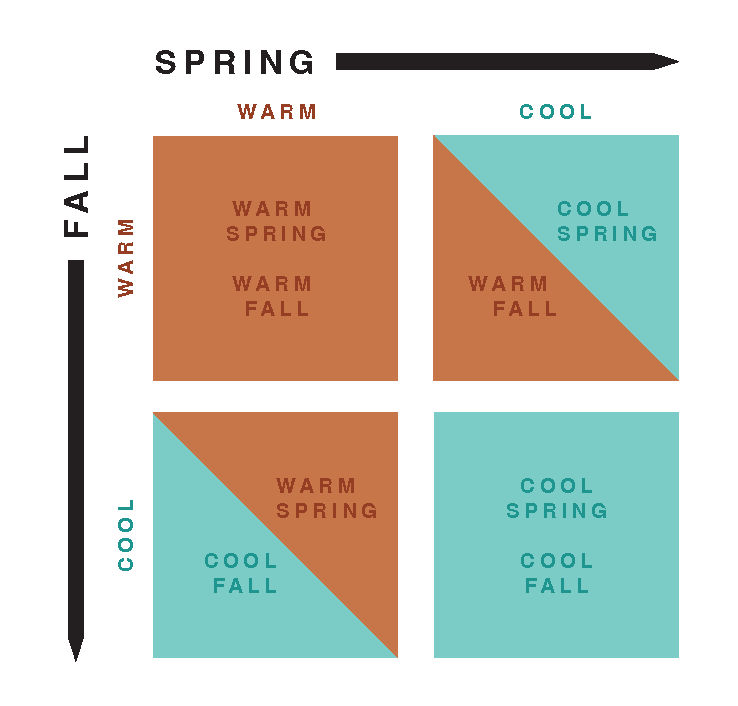
\includegraphics[width=0.7\textwidth]{FullFactorialFigure.pdf}
\caption{Arrangement of the Fuelinex four main treatments in a full factorial design}
\label{fig:fuelinexFactorial}
\end{figure}


% ============================
% Wildchrokie species
% ============================

\begin{table}[p]
\centering
\caption{Wilchrokie species grouped by tree type, life history, and wood anatomy.}
\label{tab:wildchrokieSpecies}
\begin{tabular}{|>{\raggedright\arraybackslash}p{7cm}|p{5cm}|p{3cm}|p{1cm}|}
\hline
\multicolumn{4}{|c|}{\textbf{Deciduous Trees}} \\
\hline
\textbf{Common Name (Latin)} & \textbf{Life History Strategy} & \textbf{Wood Anatomy} & \textbf{n} \\
\hline
Paper birch (\textit{Betula papyrifera}) & Fast-growth, short life  & Diffuse-porous & 8\\
Yellow birch (\textit{Betula alleghaniensis}) & Moderate-growth, moderate life & Diffuse-porous & 21\\
Grey birch (\textit{Betula populifolia}) & Fast-growth, short life & Diffuse-porous & 29\\
Grey alder (\textit{Alnus incana}) & Fast-growth, short life & Diffuse-porous & 31\\
\hline
\end{tabular}
\end{table}

% ============================
% Treespotters species
% ============================
\begin{table}[h]
\centering
\caption{Treespotters species grouped by tree type, life history, and wood anatomy.}
\label{tab:coringTreespottersSpecies}
\begin{tabular}{|>{\raggedright\arraybackslash}p{7cm}|p{5cm}|p{3cm}|p{1cm}|}
\hline
\multicolumn{4}{|c|}{\textbf{Deciduous Trees}} \\
\hline
\textbf{Common Name (Latin)} & \textbf{Life History Strategy} & \textbf{Wood Anatomy} & \textbf{n} \\
\hline
American basswood (\textit{Tilia americana}) & Fast-growth, moderate life & Diffuse-porous & 5\\
Eastern cottonwood (\textit{Populus deltoides}) & Fast-growth, short life & Diffuse-porous & 4\\
Northern red oak (\textit{Quercus rubra}) & Moderate-growth, long life & Ring-porous & 4\\
White oak (\textit{Quercus alba}) & Slow-growth, long life & Ring-porous & 5\\
Pignut hickory (\textit{Carya glabra}) & Slow-growth, long life & Ring-porous & 4\\
Shagbark hickory (\textit{Carya ovata}) & Slow-growth, long life & Ring-porous & 4\\
River birch (\textit{Betula nigra}) & Fast-growth, short life & Diffuse-porous & 5\\
Yellow birch (\textit{Betula alleghaniensis}) & Moderate-growth, moderate life & Diffuse-porous & 4\\
Sugar maple (\textit{Acer saccharum}) & Slow-growth, long life & Diffuse-porous & 5\\
Red maple (\textit{Acer rubrum}) & Slow-growth, long life & Diffuse-porous & 4\\
Yellow buckeye (\textit{Aesculus flava}) & Moderate-growth, moderate life & Diffuse-porous & 5\\
\hline
\end{tabular}
\end{table}


% --- --- --- --- --- --- --- --- --- --- --- --- --- --- --- ---
% Tables nutrient addition quantities
% --- --- --- --- --- --- --- --- --- --- --- --- --- --- --- ---
\begin{table}[h]
\centering
\caption{Nutrient addition over the two growing seasons for the nutrient addition treatment and the other treatments. The fertilizer is from Evergro (Delta, BC V4G 1B6), ID: Pepper Feed Main.}
\label{tab:nutrient}
\begin{tabular}{|l|c|c|}
\hline
\textbf{Date} & \textbf{Nutrient addition treatments} & \textbf{Regular treatments} \\
\hline
7 June 2024 & 62.5 & 62.5 \\
6 July 2024 & 62.5 & 62.5 \\
1 Sept 2024 & 250 & 0 \\
\hline
\textbf{Subtotal (2024)} & \textbf{375} & \textbf{125} \\
\hline
 &  &  \\
\hline
10 April 2025 & 0 & 125 \\
9 May 2025 & 0 & 125 \\
\textit{June 2025} & 62.5 & 62.5 \\
\textit{July 2025} & 62.5 & 62.5 \\
\hline
\textbf{Subtotal (2025)} & \textbf{125} & \textbf{375} \\
\hline
 &  &  \\
\hline
\textbf{2-year total} & \textbf{500} & \textbf{500} \\
\hline
\end{tabular}
\end{table}

% --- --- --- --- --- --- --- --- --- --- --- --- --- --- --- ---
% Tables spring frost, drought and heat waves $
% --- --- --- --- --- --- --- --- --- --- --- --- --- --- --- ---
% ============================
% Spring frost 
% ============================
\begin{table}[htbp]
\centering
\caption{Summary of late spring frosts: definition, mechanisms, trends, and consequences}
\label{tab:springFrosts}
\resizebox{\textwidth}{!}{
\begin{tabular}{|>{\raggedright\arraybackslash}p{4cm}|p{12cm}|}
\hline
\textbf{Definition:} & Late spring frosts are below-freezing temperatures in late spring \citep{zohner_late-spring_2020} \\
\hline
\textbf{Mechanisms} & Early warm spells $\rightarrow$ early leaf out $\rightarrow$ hard frost ($<$-2~$^\circ$C) $\rightarrow$ tissue death = loss of photosynthetic capacity \citep{polgar_leafout_2011}; Response: second cohort of leaves are more efficient and mitigate carbon sequestration loss \citep{reinmann_compensatory_2023} \\
\hline
\textbf{Global trend of occurrence} & Most vulnerable regions are the ones with no past risk of occurrence (); $\uparrow$ in Europe and East Asia, but $\downarrow$ in North America; global trend is controversial \citep{reinmann_compensatory_2023} \\
\hline
\textbf{Consequences (Individual and ecosystem level)} & Loss of vegetative tissue = $\downarrow$ photosynthesis = $\downarrow$ NSC and remobilization to repair damaged tissues = $\downarrow$ secondary growth \citep{meyer_frost_2024}; Loss of reproductive tissue (higher flower mortality) \citep{sgubin_risk_2018}; Economic costs for orchards \citep{reinmann_compensatory_2023} \\
\hline
\end{tabular}
}
\end{table}

\clearpage

% ============================
% Drought
% ============================
\begin{table}[htbp]
\centering
\caption{Summary of drought: definition, mechanisms, global trends, and consequences}
\label{tab:drought}
\resizebox{\textwidth}{!}{
\begin{tabular}{|>{\raggedright\arraybackslash}p{4cm}|p{12cm}|}
\hline
\textbf{Definition:} & 
``Drought is a prolonged absence or marked deficiency of precipitation that results in water shortage or a period of abnormally dry weather sufficiently prolonged for the lack of precipitation to cause a serious hydrological imbalance'' \citep{trenberth_global_2014,intergouvernemental_panel_on_climate_change_climate_2007}. \\
\hline
\textbf{Mechanisms} & 
— Hot temperature + low precipitation (global-change-type drought \citep{tyree_xylem_2002}) = $\uparrow$ evapotranspiration $\rightarrow$ less water in soil $\rightarrow$ cavitation $\rightarrow$ embolism $\rightarrow$ hydraulic failure \citep{tyree_xylem_2002} = tissue death \citep{choat_triggers_2018}; 

— Earlier spring phenology = longer GS $\rightarrow$ increased vegetative growth $\rightarrow$ increased evapotranspiration $\rightarrow$ increased drawdown of soil moisture = progressive water stress \citep{li_widespread_2023};

— Long-term vs short-term stomatal responses and consequences on tissue death \citep{choat_triggers_2018}; 

— Recovery and its determinants \citep{choat_triggers_2018,li_widespread_2023}. \\
\hline
\textbf{Global trend of occurrence} & 
— $\uparrow$ precipitation anomalies since 1990 \citep{trenberth_global_2014};  

— Climate models often exclude PDO/ENSO, limiting the attribution of increasing droughts to climate change \citep{trenberth_global_2014}; 

— Weak evidence for detection and attribution of changes in meteorological drought since the mid-20th century \citep{intergovernmental_panel_on_climate_change_detection_2014}; 

— From a spatial, model-based perspective, anthropogenic forcing increased the frequency, duration, and intensity of SPI-based droughts in North America \citep{hidalgo_detection_2009}, Europe and the Mediterranean \citep{spinoni_will_2018,kurnik_testing_2011}, and East Asia \citep{chiang_evidence_2021,marvel_twentieth-century_2019,spinoni_world_2014}. \\
\hline
\textbf{Consequences (Individual and ecosystem level)} & 
— Recurring droughts may limit trees' ability to recover from other types of stress;

— Tree mortality (e.g. Texas and California extreme droughts are estimated to have killed 300 and 102 million trees, respectively \citep{li_widespread_2023}). \\ 
\hline
\end{tabular}
}
\end{table}

\clearpage
% ============================
% Heat waves
% ============================
\begin{table}[htbp]
\centering
\caption{Summary of heat waves: definition, mechanisms, global trends, and consequences}
\label{tab:heat-waves}
\resizebox{\textwidth}{!}{
\begin{tabular}{|>{\raggedright\arraybackslash}p{4cm}|p{12cm}|}
\hline
\textbf{Definition:} & 
A heat wave is a period of excessively hot weather (five or more consecutive days during which the daily maximum temperature exceeds the long-term average maximum temperature by 5~$^\circ$C), which may be accompanied by high humidity \citep{marx_heat_2021}. \\
\hline
\textbf{Mechanisms} &  
$\uparrow$ atmospheric CO$_2$ $\rightarrow$ $\uparrow$ temperature $\rightarrow$ $\uparrow$ frequency and intensity of heat waves. More specifically, one proposed mechanism for the increased occurrence of heat waves is a weakening of the polar jet stream (a key weather driver in mid-latitude regions of North America, Europe, and Asia) caused by global warming, which increases the persistence of stationary weather patterns, resulting in prolonged heat waves or heavy rainfall events \citep{marx_heat_2021}.  

Extreme heat affects growth either (1) directly via disruption of cellular processes or (2) indirectly via increased leaf-to-air vapor pressure deficit (VPD) \citep{gagne_limited_2020}.  

Increased temperature leads to reduced photosynthesis, which can be attributed to:  
1. Damage to photosynthetic machinery;  
2. Inactivation of Rubisco;  
3. Reduced RuBP regeneration;  
4. Loss of membrane stability;  
5. Increased mitochondrial respiration and photorespiration \citep{hauck_heat_2025}. \\
\hline
\textbf{Global trend of occurrence} & 
Heat waves have increased in frequency and intensity \citep{gagne_limited_2020,meehl_more_2004,teskey_responses_2015} and are expected to increase further under future climate change \citep{dosio_extreme_2018,intergovernmental_panel_on_climate_change_detection_2014,teskey_responses_2015}.  

Summertime extreme temperatures associated with prolonged heat waves lasting several weeks now impact approximately 10\% of global land surfaces, compared to only 1\% in the 1960s \citep{teskey_responses_2015}. These trends cannot be explained solely by natural climate variability and require anthropogenic climate change \citep{marx_heat_2021}. \\
\hline
\textbf{Consequences (Individual and ecosystem level)} &  
— Reduced photosynthesis;  
— Increased mortality;  
— Loss of photosynthetic tissue \citep{gagne_limited_2020}. \\ 
\hline
\end{tabular}
}
\end{table}


\end{document}
